\documentclass[tikz,border=4pt,11pt]{standalone}
\usepackage{amsmath}
\usetikzlibrary{arrows.meta}
\definecolor{ink}{RGB}{42,52,64}
\definecolor{first}{RGB}{146,79,26}
\definecolor{second}{RGB}{26,99,111}

% Order ideals of [2]x[3] as boundary words.  The elements a=(1,1), b=(1,2),
% c=(1,3), d=(2,1), e=(2,2), f=(2,3) are drawn as cells; the ideal is shaded.
% Its upper boundary, read from the left corner to the right corner, gives a
% word with 1 for an up-right step and 0 for a down-right step.
% Left: {a,b,d} with word 01010.  Toggling the columns from left to right
% gives {a,b,c,d,e} with word 10100: the first letter moves to the end.

\begin{document}
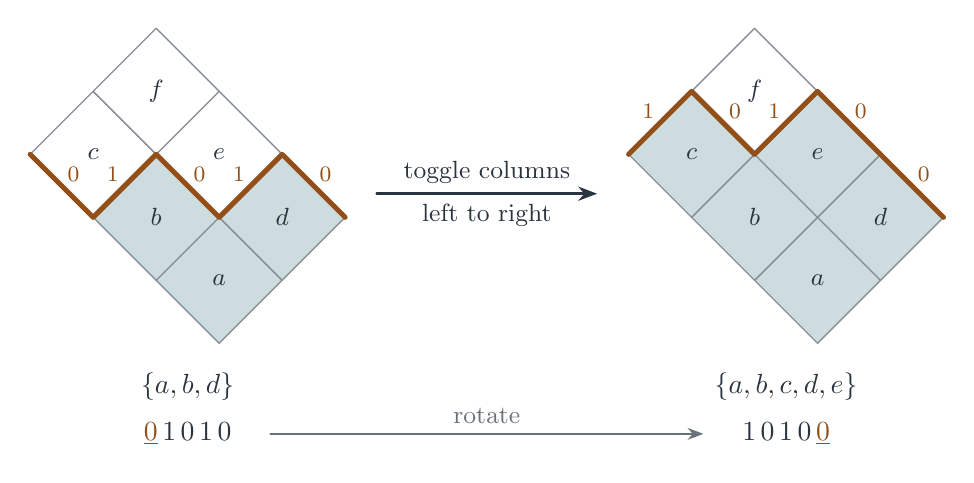
\begin{tikzpicture}[text=ink,line cap=round,line join=round]
% left: ['a', 'b', 'd'] 01010  right: ['a', 'b', 'c', 'd', 'e'] 10100
  \filldraw[fill=second!22,draw=ink!55,line width=.5pt] (0.000,0.000) -- (0.800,0.800) -- (0.000,1.600) -- (-0.800,0.800) -- cycle;
  \node[font=\small] at (0.000,0.800) {$a$};
  \filldraw[fill=second!22,draw=ink!55,line width=.5pt] (-0.800,0.800) -- (0.000,1.600) -- (-0.800,2.400) -- (-1.600,1.600) -- cycle;
  \node[font=\small] at (-0.800,1.600) {$b$};
  \filldraw[fill=white,draw=ink!55,line width=.5pt] (-1.600,1.600) -- (-0.800,2.400) -- (-1.600,3.200) -- (-2.400,2.400) -- cycle;
  \node[font=\small] at (-1.600,2.400) {$c$};
  \filldraw[fill=second!22,draw=ink!55,line width=.5pt] (0.800,0.800) -- (1.600,1.600) -- (0.800,2.400) -- (0.000,1.600) -- cycle;
  \node[font=\small] at (0.800,1.600) {$d$};
  \filldraw[fill=white,draw=ink!55,line width=.5pt] (0.000,1.600) -- (0.800,2.400) -- (0.000,3.200) -- (-0.800,2.400) -- cycle;
  \node[font=\small] at (0.000,2.400) {$e$};
  \filldraw[fill=white,draw=ink!55,line width=.5pt] (-0.800,2.400) -- (0.000,3.200) -- (-0.800,4.000) -- (-1.600,3.200) -- cycle;
  \node[font=\small] at (-0.800,3.200) {$f$};
  \draw[first,line width=1.8pt] (-2.400,2.400) -- (-1.600,1.600) -- (-0.800,2.400) -- (0.000,1.600) -- (0.800,2.400) -- (1.600,1.600);
  \node[font=\footnotesize,text=first] at (-1.850,2.150) {$0$};
  \node[font=\footnotesize,text=first] at (-1.350,2.150) {$1$};
  \node[font=\footnotesize,text=first] at (-0.250,2.150) {$0$};
  \node[font=\footnotesize,text=first] at (0.250,2.150) {$1$};
  \node[font=\footnotesize,text=first] at (1.350,2.150) {$0$};
  \filldraw[fill=second!22,draw=ink!55,line width=.5pt] (7.600,0.000) -- (8.400,0.800) -- (7.600,1.600) -- (6.800,0.800) -- cycle;
  \node[font=\small] at (7.600,0.800) {$a$};
  \filldraw[fill=second!22,draw=ink!55,line width=.5pt] (6.800,0.800) -- (7.600,1.600) -- (6.800,2.400) -- (6.000,1.600) -- cycle;
  \node[font=\small] at (6.800,1.600) {$b$};
  \filldraw[fill=second!22,draw=ink!55,line width=.5pt] (6.000,1.600) -- (6.800,2.400) -- (6.000,3.200) -- (5.200,2.400) -- cycle;
  \node[font=\small] at (6.000,2.400) {$c$};
  \filldraw[fill=second!22,draw=ink!55,line width=.5pt] (8.400,0.800) -- (9.200,1.600) -- (8.400,2.400) -- (7.600,1.600) -- cycle;
  \node[font=\small] at (8.400,1.600) {$d$};
  \filldraw[fill=second!22,draw=ink!55,line width=.5pt] (7.600,1.600) -- (8.400,2.400) -- (7.600,3.200) -- (6.800,2.400) -- cycle;
  \node[font=\small] at (7.600,2.400) {$e$};
  \filldraw[fill=white,draw=ink!55,line width=.5pt] (6.800,2.400) -- (7.600,3.200) -- (6.800,4.000) -- (6.000,3.200) -- cycle;
  \node[font=\small] at (6.800,3.200) {$f$};
  \draw[first,line width=1.8pt] (5.200,2.400) -- (6.000,3.200) -- (6.800,2.400) -- (7.600,3.200) -- (8.400,2.400) -- (9.200,1.600);
  \node[font=\footnotesize,text=first] at (5.450,2.950) {$1$};
  \node[font=\footnotesize,text=first] at (6.550,2.950) {$0$};
  \node[font=\footnotesize,text=first] at (7.050,2.950) {$1$};
  \node[font=\footnotesize,text=first] at (8.150,2.950) {$0$};
  \node[font=\footnotesize,text=first] at (8.950,2.150) {$0$};

  % words and the promotion arrow
  \node at (-0.4,-0.55) {$\{a,b,d\}$};
  \node at (-0.4,-1.15) {$\textcolor{first}{\underline{0}}\,1\,0\,1\,0$};
  \node at (7.2,-0.55) {$\{a,b,c,d,e\}$};
  \node at (7.2,-1.15) {$1\,0\,1\,0\,\textcolor{first}{\underline{0}}$};
  \draw[ink,line width=.9pt,-{Stealth[length=2.4mm]}] (2.0,1.9) -- (4.8,1.9)
    node[midway,above,font=\small] {toggle columns}
    node[midway,below,font=\small] {left to right};
  \draw[ink!70,line width=.7pt,-{Stealth[length=2mm]}] (0.65,-1.15) -- (6.15,-1.15)
    node[midway,above,font=\small] {rotate};
\end{tikzpicture}
\end{document}
